\chapter{Основной анализ}\label{ch:ch3}

В данной главе будут описаны результаты эмпирического анализа ценовых тенденций в российской экономике на основе собранных данных по ценам онлайн-ритейлеров. Отдельное внимание будет уделено вопросам базовых фактов жесткости цен, а также рассмотрено то, как характеристики ценового поведения онлайн-ритейлеров меняются во времени.

\section{Описание данных}\label{sec:ch3/sec1}

При проектировании процесса сбора данных мы также старались придерживаться принципов, описанных в работе \cite{cavallo2016billion}. Прежде всего стоит отметить, что, аналогично подходу из упомянутой работы мы сосредоточились на сборе данных с сайтов самих магазинов, а не с сайтов-агрегаторов (или маркетплейсов). Этот подход оказался технически более сложным, но обеспечивающим актуальность цен и исключающим ошибки в других характеристиках, связанных с товаром.

Методика сбора данных состояла из нескольких этапов. На первом этапе были определены необходимые для последующего анализа товары и услуги. Следует отметить, что рынок онлайн-ритейла несмотря на свой бурный рост все еще ограничен с точки зрения географии и представленности различных товаров и услуг, что наложило отпечаток на характеристики выборки.

Мы отобрали ритейлеров, продающих товары как через интернет, так и в традиционных точках продаж. Лишь небольшая часть выбранных ритейлеров специализируется исключительно на онлайн-торговле. При выборе ритейлеров мы ориентировались на следующие критерии:
\begin{itemize}
	\item занимаемая доля рынка;
	\item охват по регионам;
	\item количество охватываемых ритейлером категорий продуктов.
\end{itemize}
Продовольственные и непродовольственные ритейлеры представлены крупнейшими онлайн-ритейлерами в своих сферах:
В качестве представителей продуктовых ритейлеров были отобраны следующие:

1) гипермаркет «Перекресток» (после 2021 г. - "Впрок");
2) гипермаркет «Глобус»;
3) гипермаркет «Окей»;
4) интернет-гипермаркет «Утконос».

В качестве представителей непродовольственных ритейлеров были выбраны:
1) интернет-магазин «Lamoda»;
2) интернет-магазин «Ozon.ru»;
3) интернет-магазин «Piluli.ru».

Сфера услуг представлена несколькими местными игроками рынка, которые специализируются на пассажирских перевозках, связи, жилищно-коммунальном хозяйстве, а также рядом небольших компаний, предлагающих услуги по ремонту обуви, посещению бани и парикмахерским услугам.

Несмотря на ограниченную географию сбора данных — Москва и Московский регион — полученная информация является достаточно репрезентативной. Например, в 2021 году доля «Впрок» составила 4,5\% от общего объема интернет-торговли в Москве~\cite{X5DigitalSales2021}, а «Ozon.ru» по состоянию на 2021 год занимал второе место среди крупнейших интернет-ритейлеров России~\cite{Top100Ecommerce2021}.

С сайтов интернет-ритейлеров нами извлекались различные характеристики товаров. Специальный скрипт, написанный на языке Python, запускался на ежедневной основе и сканировал разметку продуктовых страниц с товарами, представленными на сайтах онлайн-ритейлеров (пример части продуктовой страницы представлен на рис.~\cref{fig:example_product}).

\begin{figure}[ht]
	\centerfloat{
		
\includegraphics[width=\textwidth, keepaspectratio]{example_product}
	}
	\caption{Условный пример страницы с товаром}\label{fig:example_product}
\end{figure}


Собранные данные включали информацию о дате сбора, названии товара, единице измерения, цене продажи и старой цене в случаях, когда товар продавался со скидкой (пример собранной информации представлен в таблице~\ref{tab:product_data}). Наличие информации о  особенно важно, поскольку для построения индексов цен, согласно официальной методологии Росстата, учитываются только регулярные цены (т.е. не цены распродаж). Кроме того, тенденции в доле распродажных цен от общего числа цен могут служить важным индикатором общего макроэкономического состояния в стране~\cite{Nakamura2008}. 

\begin{table}[h!]
	\centering
	\caption{Пример структуры данных о товарах}
	\label{tab:product_data}
	\scriptsize
	\begin{tabular}{|c|c|p{4cm}|c|c|c|c|c|}
		\hline
		\textbf{id} & \textbf{date} & \textbf{site\_title} & \textbf{category\_id} & \textbf{site\_code} & \textbf{site\_unit} & \textbf{posted\_price} & \textbf{sale} \\ \hline
		0 & 28.10.2019 & Молоко ЭкоНива ультрапастеризованное 3.2\% 1л & 22 & globus & 1 шт. & 77.99 & 1 \\ \hline
		1 & 28.10.2019 & Печенье Любятово Мария традиционное 156г & 29 & globus & 1 шт. & 184.99 & 0 \\ \hline
		2 & 28.10.2019 & Чай чёрный Greenfield Earl Grey Fantasy, 25×2 г & 31 & globus & 1 уп. & 85.99 & 0 \\ \hline
		\vdots & \vdots & \vdots & \vdots & \vdots & \vdots & \vdots & \vdots \\ \hline
	\end{tabular}
\end{table}


Собранные данные охватывают 33 категории продовольственных товаров, 38 категорий непродовольственных товаров и 6 категорий услуг. Следует отметить, что в данном исследовании термин «категория» обозначает совокупность товаров или услуг определённого вида (например, «Печенье»). Термин «позиция» используется для обозначения конкретного представителя данной совокупности (например, «Печенье Merba Два шоколада 200~г»).

При отборе категорий мы ориентировались на фиксированный набор товаров и услуг, используемый Росстатом, которые имеют высокий спрос среди населения и являются значимыми индикаторами при определении минимального размера оплаты труда. Некоторая узость набора товаров и услуг по сравнению с индексом потребительских цен (ИПЦ) объясняется ограниченными ресурсами, доступными на момент запуска нами автоматизированного сбора данных.

Как было упомянуто ранее, мы собрали информацию о ценах на 33 категории продуктов питания, которые входят в условный (минимальный) набор товаров, регулярно фиксируемый Росстатом каждый месяц (см. таблицу \ref{tab:food_categories}). Этот набор включает основные продукты, потребляемые большей частью населения, и поэтому имеет высокую социальную значимость. В целом наибольшая полнота с точки зрения длины и непрерывности рядов данных отмечается для продовольственных категорий. Наш опыт показал, что многие базовые продовольственные товары остаются «на полке» в течение долгого времени и почти не подвержены временному отсутствию.

\begin{longtable}{p{0.5cm} p{3.5cm} p{3.5cm} p{3cm}} % Уменьшение ширины столбцов
	\caption{Перечень продовольственных категорий, составляющих условный (минимальный) набор продуктов питания Росстата} \label{tab:food_categories} \\
	\toprule
	\textbf{№ п/п} & \textbf{Название категории} & \textbf{Единица измерения} & \textbf{Вес (количество) товара в год} \\
	\midrule
	\endfirsthead
	
	\toprule
	\textbf{№ п/п} & \textbf{Название категории} & \textbf{Единица измерения} & \textbf{Вес (количество) товара в год} \\
	\midrule
	\endhead
	
	\endfoot
	
	\endlastfoot
	
	\footnotesize % Уменьшение размера текста на большее значение
	1   & Говядина (кроме бескостного мяса) & кг & 15 \\
	2   & Свинина (кроме бескостного мяса) & кг & 4 \\
	3   & Баранина (кроме бескостного мяса) & кг & 1,8 \\
	4   & Куры охлажденные и мороженые & кг & 14 \\
	5   & Рыба мороженая неразделанная & кг & 14 \\
	6   & Сельдь соленая & кг & 0,7 \\
	7   & Масло сливочное & кг & 1,8 \\
	8   & Масло подсолнечное & кг & 7 \\
	9   & Маргарин & кг & 6 \\
	10  & Молоко питьевое цельное пастеризованное 2,5 - 3,2\% жирности & л & 110 \\
	11  & Сметана & кг & 1,8 \\
	12  & Творог нежирный & кг & 10 \\
	13  & Сыры сычужные твердые и мягкие & кг & 2,5 \\
	14  & Яйца куриные & 10 шт. & 18 \\
	15  & Сахар-песок & кг & 20 \\
	16  & Мука пшеничная & кг & 20 \\
	17  & Хлеб из ржаной муки и из смеси муки ржаной и пшеничной & кг & 115 \\
	18  & Хлеб и булочные изделия из пшеничной муки 1 и 2 сортов & кг & 75 \\
	19  & Рис шлифованный & кг & 5 \\
	20  & Пшено & кг & 6 \\
	21  & Горох и фасоль & кг & 7,3 \\
	22  & Вермишель & кг & 6 \\
	23  & Картофель & кг & 150 \\
	24  & Капуста белокочанная свежая & кг & 35 \\
	25  & Морковь & кг & 35 \\
	26  & Огурцы свежие & кг & 1,8 \\
	27  & Лук репчатый & кг & 20 \\
	
\end{longtable}

\newpage % Переход на новую страницу

\noindent
\textbf{Продолжение таблицы \ref{tab:food_categories}:} \\

\begin{longtable}{p{0.5cm} p{3.5cm} p{3.5cm} p{3cm}} % Уменьшение ширины столбцов
	\toprule
	\textbf{№ п/п} & \textbf{Название категории} & \textbf{Единица измерения} & \textbf{Вес (количество) товара в год} \\
	\midrule
	\endfirsthead
	
	\toprule
	\textbf{№ п/п} & \textbf{Название категории} & \textbf{Единица измерения} & \textbf{Вес (количество) товара в год} \\
	\midrule
	\endhead
	
	\endfoot
	
	\endlastfoot
	
	\footnotesize % Уменьшение размера текста на большее значение
	28  & Яблоки & кг & 18,6 \\
	29  & Печенье & кг & 0,7 \\
	30  & Карамель & кг & 0,7 \\
	31  & Чай черный байховый & кг & 0,5 \\
	32  & Соль поваренная пищевая & кг & 3,65 \\
	33  & Перец черный (горошек) & кг & 0,73 \\
	
\end{longtable}

Всего в базе содержится 2257 уникальных товаров, цены на которые регистрировались в разные периоды. Самые длительные временные ряды начинаются с января 2019 года, а самые короткие — с июня того же года. Данные по продовольственным товарам охватывают период с 31 января 2019 года по 1 октября 2024 года. Непродовольстенные товары обладают в целом значительно меньшими периодами «жизни» на сайте и в выборке охватывают период с 12 февраля 2019 года по 2 июня 2022 года. Наконец, цены на услуги доступы за период с 18 февраля 2019 года по 30 июня 2022 года.

В начале сбора данных ежедневное количество уникальных позиций товаров и услуг составляло 546 позиций, в конце – 370 позиций. Максимальное число позиций, собираемых в день за рассматриваемый период, составило 2110 (рис.~\cref{fig:count_obs}).

\begin{figure}[ht]
	\centerfloat{
		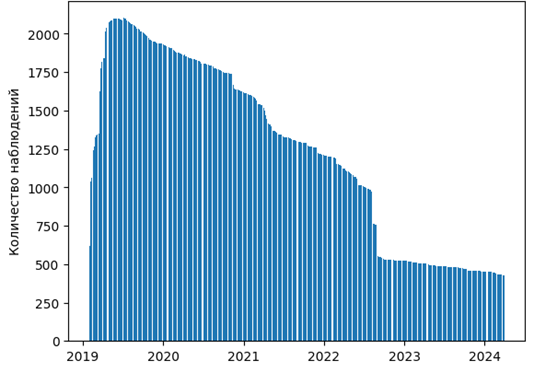
\includegraphics[scale=1]{count_obs}
	}
	\caption{Количество ежедневных наблюдений}\label{fig:count_obs}
\end{figure}

Поскольку сбор данных начался за год до начала пандемии COVID-19 и продолжается до настоящего времени, у нас есть возможность изучить отличительные характеристики различных периодов: острой фазы пандемии (первая половина 2020 года), постепенного снятия ограничений (2021 год), а также тенденции, произошедшие после введения ограничительных мер в отношении России в 2022 году.

Наличие информации о единице измерения товара позволило нам произвести дополнительную проверку того, насколько собираемые нами данные соответствуют динамике цен офлайн-ритейлеров. Так, наличие этой информации позволило рассчитать стоимость условного (минимального) набора продуктов по данным онлайн-ритейлеров и сопоставить ее со стоимостью аналогичного набора, стоимость которого отслеживается Росстатом по отдельным городам. Чтобы рассчитать стимость такого набора, мы брали 25 перцентиль стоимости внутри категории продуктов и умножали на норму потребления (табл.~ \ref{tab:food_categories}). Выбор 25 перцентиля объясняется тем, что Росстат рассматривает в своей статистике марки товаров, которые наиболее популярны среди населения, и, следовательно, собираемые данные по ценам на товары, вероятно, должны быть недорогими и доступными большинству людей.

На рисунке~\cref{fig:basket_plot} представлены графики стоимости таких наборов на основе данных по ценам онлайн-ритейлеров и данным, представленным на сайте Росстата для г. Москвы за период с 2019 по 2022 гг. Визуально динамика между стоимостями наборов является достаточно близкой, что можно объяснить следованием принципов сбора репрезентативных данных из работы \cite{cavallo2016billion}. Важную роль сыграл отбор преимущественно мультиканальных ритейлеров и ручной отбор конкретных марок продуктов, что позволило максимально приблизиться к официальной методологии Росстата.

Более формальным подтверждением наличия связи между наборами является оценка корреляции между стоимостями наборов. Значение этой оценки для очищенных от тренда рядов составила 0,82, что свидетельствует о наличии сильной линейной связи в динамике стоимостей наборов.

\begin{figure}[ht]
	\centerfloat{
		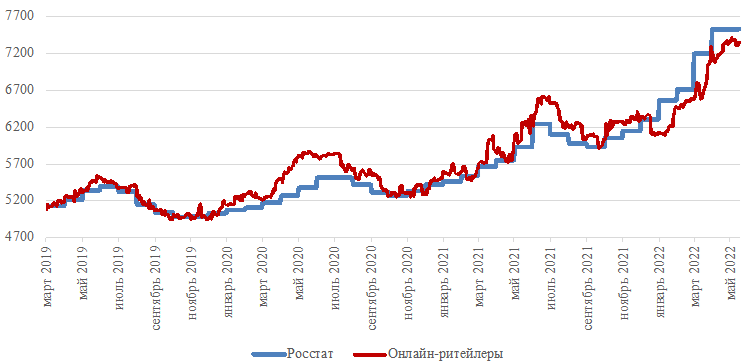
\includegraphics[width=\textwidth, keepaspectratio]{basket_plot}
	}
	\caption{Стоимость условного (минимального) набора продуктов по данным Росстата и онлайн-данным для г. Москвы (руб.)}\label{fig:basket_plot}
\end{figure}

Стоит отметить, что мы видим расхождение в динамике стоимостей наборов после марта 2020 года (и до, приблизительно, сентября) по сравнению с динамикой в 2019 году. Стоимость набора продуктов онлайн-ритейлеров стала расти существенно быстрее, чем стоимость набора по данным Росстата. Такое резкое удорожание объясняется введением локдауна в Москве и связанным с этим шоком спроса на доставку продуктов на дом. Таким образом, этот случай расходится с тем, что было получено в работе \cite{hillen2021covid}, где автор показала что существенного удорожания продуктов на данных Amazon Fresh после введения карантинных ограничений не произошло. 

\section{Базовые эмпирические факты жесткости цен в онлайн-ритейле}\label{sec:ch3/sec2}

В данной главе будут рассмотрены стилизованные факты, касающиеся жесткости цен на данных онлайн-ритейлеров. Интерес представляет сопоставление результатов, полученных по г. Москве, с данными близких зарубежных исследований, а также сопоставление с жесткостью цен в традиционных офлайн-магазинах. Кроме того, будет рассмотрено сравнение жесткости цен в периоды относительной стабильности и нестабильности в российской экономике.

Следует сказать об основных показателях, которые нами будут использоваться в анализе. Основным показателем является частота изменения цен:
\begin{equation}
	\label{eq:equation_freq}
	f=\frac{m}{M},
\end{equation}
где \( m \) "--- число периодов, в которых цена изменялась, \( M \) "--- общее число периодов наблюдения.

Иным способом измерения жесткости цен является оценка дюрации, или периода неизменности цен. Дюрация - показатель, являющийся расчетным от частоты изменения цен и показывающий в течение какого времени цена на товар или услугу остается неизменной:
\begin{equation}
	\label{eq:equation_duration}
	D_k^{av}=\frac{-1}{ln⁡(1-F_k)},
\end{equation}
где \( k \) "--- идентификатор категории товара, \( F_k \) "--- средняя частота изменения. Показатель дюрации является более интерпретируемым, посколько показывает количество дней, в течение которых цена остается неизменной.

В таблице 11 представлены результаты оценки средней частоты изменения цен по используемой нами выборке с 2019 по 2022 гг. Средняя частота была рассчитана как доля изменённых цен от общего числа товаров внутри категории (в день). Анализ показывает значительную неоднородность частот между продовольственными, непродовольственными категориями товаров, а также среди отдельных категорий услуг. 

Среди продовольственных товаров (табл.~\ref{tab:products}) наиболее высокой частотой изменения цен характеризуются сезонные продукты. Так, для картофеля этот показатель составил в среднем 7,17\% в день, для огурцов — 6,75\%, яблок — 6,64\%, капусты — 4,98\%, моркови — 4,69\% и репчатого лука — 4,56\%. Сезонный характер предложения этих товаров приводит к их высокой волатильности и, как следствие, частым изменениям цен. 

\begin{longtable}{|p{1cm}|p{8.5cm}|p{3.5cm}|p{3cm}|} % Уменьшение ширины столбцов
	\caption{Средние частоты и дюрации: Продовольственные товары} \label{tab:products} \\
	\hline
	\textbf{№ п/п} & \textbf{Наименование категории} & \textbf{Средняя частота (\% в день)} & \textbf{Средняя дюрация (дней)} \\
	\hline
	\hline
	\endfirsthead
	
	\hline
	\textbf{№ п/п} & \textbf{Наименование категории} & \textbf{Средняя частота (\% в день)} & \textbf{Средняя дюрация (дней)} \\
	\hline
	\hline
	\endhead
	
	\hline
	\endfoot
	
	\hline
	\endlastfoot
	
	\footnotesize % Уменьшение размера текста на большее значение
	1   & Баранина (кроме бескостного мяса) & 1,13 & 88,0 \\
	2   & Говядина (кроме бескостного мяса) & 0,76 & 73,6 \\
	3   & Пшено & 1,73 & 57,3 \\
	4   & Рыба мороженая неразделанная & 1,97 & 50,3 \\
	5   & Горох и фасоль & 2,27 & 43,6 \\
	6   & Хлеб и булочные изделия из пшеничной муки 1 и 2 сортов & 2,32 & 42,6 \\
	7   & Свинина (кроме бескостного мяса) & 2,51 & 39,3 \\
	8   & Сахар-песок & 2,63 & 37,5 \\
	9   & Сыры сычужные твердые и мягкие & 2,81 & 35,1 \\
	10  & Рис шлифованный & 2,81 & 35,1 \\
	11  & Карамель & 2,92 & 33,7 \\
	12  & Сельдь соленая & 2,97 & 33,2 \\
	13  & Соль поваренная пищевая & 3,2 & 30,7 \\
	14  & Печенье & 3,29 & 29,9 \\
	15  & Вермишель & 3,59 & 27,4 \\
	16  & Маргарин & 3,59 & 27,4 \\
	17  & Куры охлажденные и мороженые & 3,6 & 27,3 \\
	18  & Крупа гречневая-ядрица & 3,63 & 27,0 \\
	19  & Мука пшеничная & 3,66 & 26,8 \\
	20  & Чай черный байховый & 3,69 & 26,6 \\
	21  & Перец черный (горошек) & 3,71 & 26,5 \\
	22  & Яйца куриные & 3,76 & 26,1 \\
	23  & Молоко питьевое цельное пастеризованное 2,5--3,2\% жирности & 3,86 & 25,4 \\
	24  & Масло сливочное & 3,88 & 25,3 \\
	25  & Творог нежирный & 3,92 & 25,0 \\
	26  & Хлеб из ржаной муки и из смеси муки ржаной и пшеничной & 3,98 & 24,6 \\
	27  & Сметана & 4,03 & 24,3 \\
	28  & Масло подсолнечное & 4,51 & 21,7 \\
	29  & Лук репчатый & 4,56 & 21,4 \\
	30  & Морковь & 4,69 & 20,8 \\
	31  & Капуста белокочанная свежая & 4,98 & 19,6 \\
	32  & Яблоки & 6,64 & 14,6 \\
	33  & Огурцы свежие & 6,75 & 14,3 \\
	34  & Картофель & 7,17 & 13,4 \\
	
\end{longtable}

Среди непродовольственных товаров (таб.~\ref{tab:non_food_products}) максимальная частота изменения цен наблюдается у лекарственных препаратов. Например, для корвалола она составила 8,84\%, а для анальгина — 7,22\%. Такая высокая частота изменений цен может быть связана как с сезонными вспышками простудных заболеваний, так и с эпидемическими волнами, провоцирующими резкий рост спроса на данные препараты.

\begin{longtable}{|p{1cm}|p{8.5cm}|p{3.5cm}|p{3cm}|} % Задаем ширину столбцов
	\caption{Средние частоты и дюрации: Непродовольственные товары}
	\label{tab:non_food_products} \\
	\hline
	\textbf{№ п/п} & \textbf{Наименование категории} & \textbf{Средняя частота (\% в день)} & \textbf{Средняя дюрация (дней)} \\
	\hline
	\hline
	\endfirsthead
	
	\hline
	\textbf{№ п/п} & \textbf{Наименование категории} & \textbf{Средняя частота (\% в день)} & \textbf{Средняя дюрация (дней)} \\
	\hline
	\hline
	\endhead
	
	\hline
	\endfoot
	
	\hline
	\endlastfoot
	
	35 & Джемпер для детей школьного возраста & 0,02 & 4 999,5 \\ \hline
	36 & Кроссовые туфли для детей с верхом из искусственной кожи & 0,06 & 1 666,2 \\ \hline
	37 & Брюки для детей школьного возраста из джинсовой ткани & 0,07 & 1 428,1 \\ \hline
	... & Добавьте остальные строки для непродовольственных товаров & ... & ... \\ \hline
	69 & Метамизол натрия (Анальгин отечественный) & 7,22 & 13,3 \\ \hline
	
\end{longtable}

Услуги (таб.~\ref{tab:services}), напротив, характеризуются сравнительно низкой частотой изменения цен. Это объясняется высокой долей трудовых издержек в их стоимости и более редким пересмотром цен трудовых контрактов по сравнению с сырьём. Заработная плата, являясь основной составляющей трудовых издержек, обычно фиксируется в трудовом договоре и остается неизменной на протяжении определенного периода \cite{Vermeulen2012}.

\begin{longtable}{|p{1cm}|p{8.5cm}|p{3.5cm}|p{3cm}|} % Ширина столбцов оптимизирована
	\caption{Средние частоты и дюрации: Услуги}
	\label{tab:services} \\
	\hline
	\textbf{№ п/п} & \textbf{Наименование категории} & \textbf{Средняя частота (\% в день)} & \textbf{Средняя дюрация (дней)} \\
	\hline
	\hline
	\endfirsthead
	
	\hline
	\textbf{№ п/п} & \textbf{Наименование категории} & \textbf{Средняя частота (\% в день)} & \textbf{Средняя дюрация (дней)} \\
	\hline
	\hline
	\endhead
	
	\hline
	\multicolumn{4}{r}{Продолжение на следующей странице} \\
	\hline
	\endfoot
	
	\hline
	\endlastfoot
	
	71 & Постановка набоек & 0 &  \\ \hline
	72 & Стрижка модельная в женском зале & 0,06 & 1 666,2 \\ \hline
	73 & Абонентская плата за неограниченный объем местных телефонных соединений & 0,14 & 713,8 \\ \hline
	74 & Помывка в бане в общем отделении & 0,16 & 624,5 \\ \hline
	75 & Проезд в городском муниципальном автобусе & 0,30 & 332,8 \\ \hline
	76 & Проезд в троллейбусе & 0,32 & 312,0 \\ \hline
	
\end{longtable}

В таблице \ref{tab:comparison} приведено сравнение наших оценок жесткости цен и среднего размера изменений цен с данными исследования \cite{cavallo2018scraped}, проведенного среди онлайн-ритейлеров США, Аргентины, Бразилии, Чили и Колумбии. Для обеспечения сопоставимости мы рассчитали среднюю продолжительность неизменности цен (дюрацию) на основе средней частоты изменения всех цен (включая распродажи) в наших еженедельных данных. Как видно из таблицы, оценка дюрации в России оказалась значительно ниже, чем в \cite{cavallo2018scraped}, что указывает на более частые изменения цен в России по сравнению с указанными странами. Это может быть связано с двумя факторами. Во-первых, в нашей выборке преобладают продовольственные товары, которые, как правило, меняются чаще, чем непродовольственные (см., например, \cite{bils2004some}). Во-вторых, в 2022 году (который включен в наши расчеты) в России наблюдался резкий рост инфляции, что также могло привести к увеличению частоты изменения цен по сравнению с зарубежными странами.

Кроме того, из таблицы видно, что средний размер изменений цен в России ниже, чем в сравниваемых странах. Это объясняется тем, что в исследуемый период инфляция в нашей выборке была относительно низкой, что позволяло ритейлерам изменять цены постепенно и на небольшие величины.

\begin{table}[h]
	\centering
	\small % Уменьшение размера шрифта
	\caption{Сопоставление результатов по средней дюрации и размеру изменений цен с зарубежными оценками из работы \cite{cavallo2018scraped}}
	\label{tab:comparison}
	\begin{tabularx}{\textwidth}{|X|X|X|X|X|X|X|} % Использование tabularx с шириной \textwidth
		\hline
		Показатель & Наши результаты за 2019–2022 гг. & \multicolumn{5}{c|}{Результаты \cite{cavallo2018scraped} за период с 2007 по 2010 гг.} \\
		\cline{3-7}
		&  & США & Аргентина & Бразилия & Чили & Колумбия \\
		\hline
		Дюрация (среднее, недель) & 1,1 & 2,9 & 2,4 & 1,5 & 2,9 & 2,0 \\
		\hline
		Средний размер изменений по модулю & 6,7 & 22,0 & 12,2 & 11,5 & 14,7 & 10,7 \\
		\hline
	\end{tabularx}
\end{table}

% частота изменения цен - общая и по отдельным товарам - продам, непродам и услугам
% можно сразу написать о том, какие результаты были получены на зарубежных исследованиях по онлайн-ценам - Lunneman, Wintr 2011, Cavallo 2018
%% описать показатели жесткости цен
% 

Отдельного внимания заслуживает наличие сезонности в изменениях цен. Такая сезонность может иметь значение для мер воздействия денежно-кредитной политики на экономику. Так, в работе \cite{olivei2007} было показано, что реакция выпуска на монетарные шоки, идентифицированные с помощью структурной VAR-модели, оказывается сильнее для шоков, происходящих в первом и втором кварталах, по сравнению с шоками, происходящими в третьем и четвертом кварталах. Эмпирические данные по США потверждают эти выводы: так, в работе \cite{Nakamura2008} на месячных данных авторы рассчитали, что частота изменения цен в первом квартале составляет 15,9\%, но снижается до всего лишь 8,2\% в четвертом квартале. Для цен производителей большая часть сезонности объясняется резким скачком частоты изменения цен в январе. В работе \cite{alvarez2006sticky} обнаруживают схожие закономерности для потребительских цен в зоне евро.

Наши результаты (рис. \ref{fig:seasonality}) показывают, что наибольшая доля изменений приходится на второе полугодие, а именно на ноябрь-декабрь. Во многом такое поведение ритейлеров объясняется количеством изменений цен, ассоциированных с распродажами и связанными с этим подстройками цен для более эффективной конкуренции.

\begin{figure}[h]
	\centering
	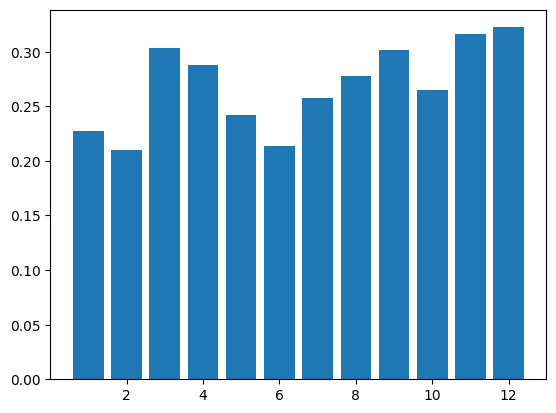
\includegraphics[width=0.8\textwidth]{seasonality.png} % Укажите путь к изображению и настройте ширину
	\caption{Частота изменения цен по месяцам} % Подпись к изображению
	\label{fig:seasonality} % Метка для ссылок в тексте
\end{figure}
 

\section{Соответствие эмпирических фактов теоретическим моделям ценообразования}\label{sec:ch3/sec3}

	
В 1980-е годы были разработаны различные теоретические модели ценообразования, объясняющие медленную подстройку цен. Эти модели делятся на два основных класса: модели, в которых изменение цен происходит с заданной периодичностью (time-dependent models) \cite{Calvo1983, Taylor1980}, и модели, в которых решение о корректировке цен зависит от состояния экономики (state-dependent models) \cite{CaplinSpulber1987, Dotsey1999, Rotemberg1982}. 

В моделях, зависящих от времени, жесткость цен объясняется наличием фиксированных трудовых контрактов, ограничивающих возможность изменения цен определенными моментами времени. Напротив, в моделях, зависящих от состояния экономики, фирмы могут корректировать цены в любой момент, однако такие изменения сопряжены с издержками. Если ожидаемая выгода от изменения цены не превышает эти издержки, фирма сохраняет цены неизменными. Таким образом, механизмы ценовой жесткости существенно различаются в разных моделях, и выбор соответствующей модели ценообразования играет важную роль в точности прогнозирования экономических последствий шоков.

Общим свойством моделей, зависящих от времени, является экзогенно заданный момент изменения цен. Фирмы устанавливают новые цены либо через фиксированные интервалы времени \cite{Taylor1980}, либо случайным образом \cite{Calvo1983}, игнорируя текущую экономическую ситуацию. Наиболее распространёнными моделями этого класса являются модель Тэйлора \cite{Taylor1980} и модель Кальво \cite{Calvo1983}.

Позднее такие модели подверглись критике за предположение об экзогенной периодичности изменения цен. В частности, фирмы в этих моделях не учитывают макроэкономические условия при выборе момента пересмотра цен, что противоречит эмпирическим наблюдениям, особенно в периоды высокой инфляции \cite{Barros2009, gagnon2009, NyawoRankin2016}.

В отличие от моделей, зависящих от времени, модели, основанные на состоянии экономики, предполагают, что стимулы к изменению цен возрастают в периоды высокой инфляции. Здесь решение о корректировке цен принимается эндогенно, исходя из рыночных условий. В условиях экономического шока фирмы, изменившие цены ранее, получают больше выгоды, поскольку накопленная инфляция увеличивает разрыв между желаемой и фактической ценой \cite{Dotsey1999, golosov2007}. Следует отметить, что модели, основанные исключительно на времени или на состоянии экономики, не всегда соответствуют эмпирическим данным. Это привело к разработке гибридных моделей, сочетающих элементы обоих подходов \cite{Nakamura2008}, что позволяет лучше объяснять реальные ценовые динамики.

Результаты зарубежных эмпирических исследований (\cite{gagnon2009, KlenowKryvtsov2008} и др.) показывают, что выводы о соответствии наблюдаемых фактов не всегда можно отнести к одной из моделей ценообразования. Эти различия проявляются между развитыми и развивающимися экономиками, в периоды высокой и низкой инфляции, а также зависят от источника данных. В этом контексте особый интерес представляет изучение ценовых механизмов в России.

Как было отмечено раннее, в нашем наборе данных наблюдается гетерогенность в жесткости цен между отдельными товарами и услугами (таб.~\ref{tab:products}, \ref{tab:non_food_products}, \ref{tab:services}), что можно объяснить разной долей трудовых издержек в конечной цене товара.

Еще одной важной характеристикой ценообразования онлайн-ритейлеров является распределение изменений цен и наличие «тяжёлых» хвостов в этом распределении (рис. \ref{fig:hist}). Значение куртозиса  (коэффициента эксцесса) для распределения цен без исключения распродаж оказалось равным 11, с исключением распродаж — 17. Для сравнения: в нормальном распределении значение куртозиса равно трем. Высокое значение куртозиса говорит о том, что имеется существенная часть изменений на небольшую в абсолютном выражении величину.

\begin{figure}[h!]
	\centering
	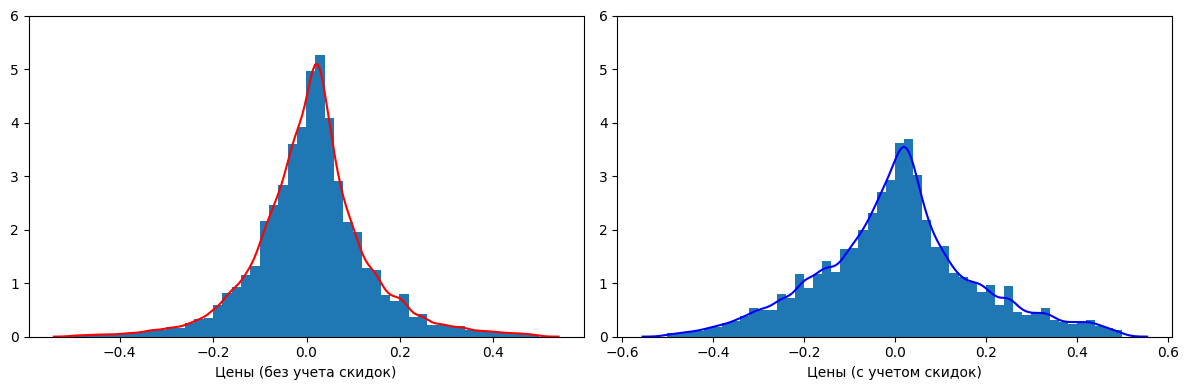
\includegraphics[width=\textwidth]{hist.png} % Укажите путь к вашему изображению
	\caption{Гистограмма и KDE для цен с учетом и без учета скидок}
	\label{fig:hist}
\end{figure}


В исследованиях, проведённых по США \cite{KlenowMalin2010, Midrigan2011}, также отмечается, что значительная часть всех изменений цен приходится на малые корректировки. В частности, согласно \cite{KlenowKryvtsov2008}, в США 44\% всех изменений цен (исключая распродажи) не превышают 5\% по амплитуде, 25\% — менее 2,5\%, а 12\% — менее 1\%. Высокая доля изменений цен, не превышающих 1\%, указывает на одномодальность распределения. Однако в работе \cite{cavallo2018scraped} утверждается, что этот вывод может быть ошибочным из-за частых замен пропущенных наблюдений аналогичными товарами, что характерно для данных, используемых при расчёте индекса потребительских цен. Таким образом, в действительности доля изменений менее 1\% может быть значительно ниже, что свидетельствует о наличии определённых издержек, препятствующих фирмам проводить слишком малые изменения цен.


Наш результат показал, что по абсолютной величине цены в среднем меняются на 6,7\%. Было также рассчитана доля изменений цен ниже определённых порогов, как с учётом распродаж, так и без них (табл. \ref{tab:small_price_changes}). Оказалось, что 34\% всех случаев изменения цен составляют колебания менее 5\%, а для регулярных цен этот показатель достигает 39\%. Несмотря на относительно высокую долю изменений ниже 5\%, изменения менее 1\% встречаются редко. Это может свидетельствовать о наличии издержек меню, что соответствует выводам некоторых моделей ценообразования, зависящих от состояния экономики \cite{golosov2007, Midrigan2011}.

\begin{table}[h]
	\centering
	\small % Уменьшение размера шрифта
	\caption{Доля небольших изменений в общем числе изменений цен}
	\label{tab:small_price_changes}
	\begin{tabularx}{\textwidth}{|X|X|X|X|} % Использование tabularx с шириной \textwidth
		\hline
		\textbf{Тип цен} & \multicolumn{3}{c|}{\textbf{Доля изменений цен (\%)}} \\
		\cline{2-4}
		& \makecell{изменения \\ менее чем на 5\% \\ по модулю} 
		& \makecell{изменения \\ менее чем на 2,5\% \\ по модулю} 
		& \makecell{изменения \\ менее, чем на 1\% \\ по модулю} \\
		\hline
		Цены без исключения распродаж & 34 & 15 & 2 \\
		\hline
		Цены с исключением распродаж & 39 & 21 & 5 \\
		\hline
	\end{tabularx}
\end{table}

% Добавить инфо о том, как менялась ситуация после 2022 года

%% Про функцию риска

Эффективным показателем с точки зрения определения того, какая из моделей ценообразования может соответствовать наблюдаемым данным, является функция риска (hazard function) (см. \cite{nakamura2013price}). Функция риска описывает вероятность изменения цены в период \( t+1 \), при условии, что цена оставалась неизменной в течение \( t \) периодов. В данном случае, функция риска, рассчитанная на основе регулярных цен (как показано на рис.~\ref{fig:risk_function}), демонстрирует явный убывающий характер: чем дольше цена остается неизменной, тем ниже вероятность её изменения в следующий период.

Этот результат согласуется с выводами других исследований. Например, аналогичная зависимость была обнаружена в работе \cite{Nakamura2008} на основе данных по США, а также в исследовании \cite{cavallo2018scraped}, где анализировались данные из четырех латиноамериканских стран. Таким образом, убывающий характер функции риска изменения цены является устойчивой закономерностью, наблюдаемой в разных экономиках.

\begin{figure}[h!]
	\centering
	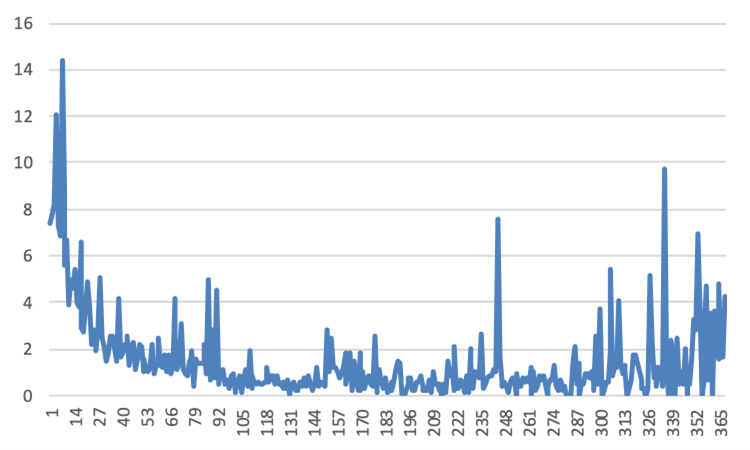
\includegraphics[width=0.8\textwidth]{risk_function.png} % Укажите путь к вашему изображению
	\caption{Функция риска для цен без учета распродаж (ось \( y \) - доля изменившихся цен от всех цен, ``доживших'' до данного дня, ось \( x \) - продолжительность периода (в днях) с последнего изменения цены)}
	\label{fig:risk_function}
\end{figure}

Основной причиной убывающего характера функции риска является гетерогенность в частотах изменения цен между различными категориями товаров и услуг \cite{Nakamura2008}. Это связано с тем, что в выборке присутствуют товары с разной степенью ценовой гибкости: одни имеют жесткие цены (меняются редко), а другие --- гибкие цены (меняются часто). Средняя частота изменения цен в каждом периоде зависит от соотношения товаров с жесткими и гибкими ценами.

Если в выборке преобладают товары с гибкими ценами, то в начальные периоды средняя частота изменения цен будет высокой, так как цены на такие товары меняются часто. Однако с течением времени доля товаров с гибкими ценами в общей массе товаров, цены на которые остались неизменными, снижается. Это происходит потому, что товары с гибкими ценами уже изменили свои цены в предыдущих периодах. В результате в последующие периоды в выборке остаются преимущественно товары с жесткими ценами, вероятность изменения которых значительно ниже. Таким образом, средняя частота изменения цен снижается с увеличением продолжительности периода неизменности цен. К последним периодам ``доживают'' в основном товары с жесткими ценами, что объясняет убывающий характер функции риска.

Одним из подходов к решению проблемы гетерогенности в частотах изменения цен является построение функции риска для более однородных групп товаров и услуг. Примеры, представленные на рис.~\ref{fig:hazard_a}, \ref{fig:hazard_b} и \ref{fig:hazard_c}, демонстрируют, что убывающий наклон функции риска сохраняется даже в этом случае. Однако при этом наблюдается более выраженная тенденция к увеличению вероятности изменения цен в более поздние периоды. Подобная тенденция характерна и для большинства других анализируемых категорий товаров и услуг.

\begin{figure}[h]
	\centering
	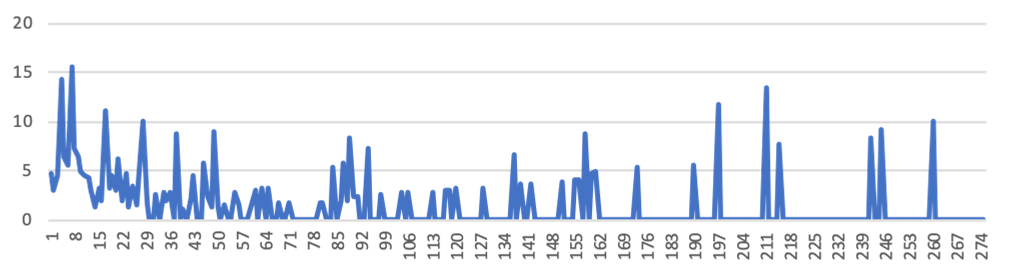
\includegraphics[width=\textwidth]{hazard_a}
	\caption{Функция риска изменения цены для категории «Рис шлифованный»}
	\label{fig:hazard_a}
\end{figure}

\begin{figure}[h]
	\centering
	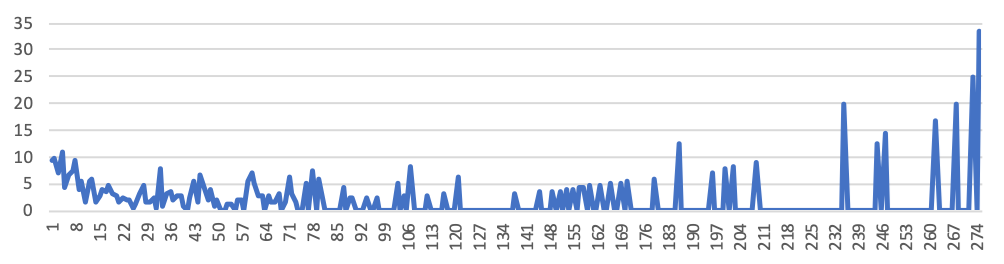
\includegraphics[width=\textwidth]{hazard_b}
	\caption{Функция риска изменения цены для категории «Сыры сычужные»}
	\label{fig:hazard_b}
\end{figure}

\begin{figure}[h]
	\centering
	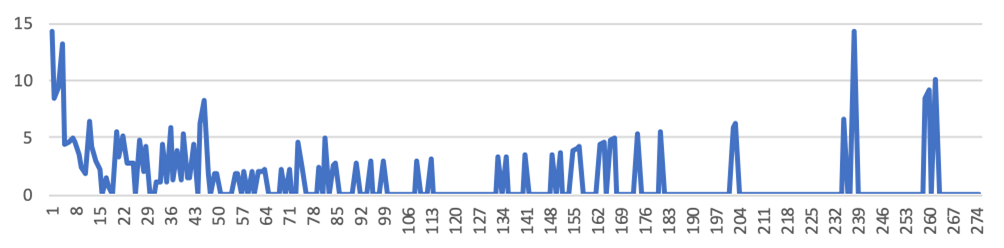
\includegraphics[width=\textwidth]{hazard_c}
	\caption{Функция риска изменения цены для категории «Горох и фасоль»}
	\label{fig:hazard_c}
\end{figure}

Одной из ключевых динамических характеристик изменения цен фирм является зависимость величины корректировки цены от продолжительности периода её неизменности. На рассматриваемом временном отрезке эта зависимость демонстрирует явный тренда (см. рис. \ref{fig:size_vs_change}). Отметим, что данный результат противоречит выводам моделей ценообразования, основанных на временных зависимостях \cite{Taylor1980, Calvo1983}, однако соответсвует выводам моделей, учитывающих состояние экономики \cite{Dotsey1999, golosov2007}. Согласно этим моделям, накопленные инфляционные шоки должны приводить к тому, что чем дольше цена остается неизменной, тем значительнее должно быть её последующее изменение.

\begin{figure}[h]
	\centering
	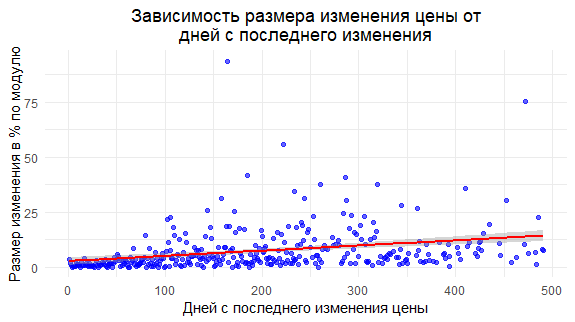
\includegraphics[width=\textwidth]{size_vs_change}
	\caption{Динамика изменения цен в зависимости от продолжительности их фиксации}
	\label{fig:size_vs_change}
\end{figure}

Для более формального обоснования мы оценили регрессию зависимости изменений цен от того, насколько долго цена оставалась неизменной:

\begin{equation}
	\mathit{change}_i = \mathit{\beta_0} + \mathit{\beta_1} \cdot \mathit{days}_i + \varepsilon_i.
	\label{eq:regression_model}
\end{equation}


Результаты оценки представлены в таб. \ref{tab:size_vs_age_reg}. Таким образом, вы видим, что количество дней неизменности является статистическим значимым фактором для размера изменений цен, что подтверждает логику влияния накопленных шоков на цены.

\begin{table}[!htbp]
	\captionsetup{justification=raggedright, singlelinecheck=false} % Выровнять заголовок по левому краю
	\caption{Оценка линейной регрессии зависимости размера изменения от продолжительности неизменности цены} 
	\label{tab:size_vs_age_reg}
	\centering
	\begin{tabular}{@{\extracolsep{5pt}}l D{.}{.}{-3} } 
		\\[-1.8ex] \hline 
		\hline \\[-1.8ex] 
		& \multicolumn{1}{c}{\textbf{Зависимая переменная:}} \\ 
		\cline{2-2} 
		\\[-1.8ex] & \multicolumn{1}{c}{\textit{Размер изменения (change)}} \\ 
		\hline \\[-1.8ex] 
		\textbf{Дни с последнего изменения (days)} & 0.023^{***} \\ 
		& (0.004) \\ 
		& \\ 
		\textbf{Константа} & 2.785^{***} \\ 
		& (0.727) \\ 
		& \\ 
		\hline \\[-1.8ex] 
		Число наблюдений & \multicolumn{1}{c}{359} \\ 
		Коэффициент детерминации R$^{2}$ & \multicolumn{1}{c}{0.089} \\ 
		Скорректированный R$^{2}$ & \multicolumn{1}{c}{0.086} \\ 
		Среднеквадратическая ошибка остатков & \multicolumn{1}{c}{9.411 (df = 357)} \\ 
		F-критерий & \multicolumn{1}{c}{34.801$^{***}$ (df = 1; 357)} \\ 
		\hline 
		\hline \\[-1.8ex] 
		\multicolumn{2}{l}{\textbf{Примечание:}} \\ 
		\multicolumn{2}{l}{$^{*}$ p$<$0.1; $^{**}$ p$<$0.05; $^{***}$ p$<$0.01 (уровень значимости)} \\ 
	\end{tabular} 
\end{table}

В исследовании \cite{Taylor1980} было подчеркнуто, что синхронность ценового поведения фирм играет ключевую роль в определении продолжительности воздействия шоков денежно-кредитной политики на реальный сектор экономики. Чем более децентрализованным и разрозненным является процесс изменения цен, тем дольше сохраняются реальные эффекты монетарных шоков. Одним из показателей степени координации ценовых изменений выступает изменчивость частоты корректировки цен во времени. 

Для эмпирической проверки данного утверждения инфляция представляется в виде произведения интенсивной (средний размер изменений цен) и экстенсивной (доля товаров, цены которых изменились в данный период) составляющих \cite{klenow2008state}:

\begin{equation}
	\pi_t = \sum_{i} w_i (p_{it} - p_{it-1}) 
	= \underbrace{\sum_{i} w_i I_{it}}_{\mathit{fr}_t}
	\cdot 
	\underbrace{\frac{\sum_{i} w_i (p_{it} - p_{it-1})}{\sum_{i} w_i I_{it}}}_{\mathit{dp}_t}
	= \mathit{fr}_t \cdot \mathit{dp}_t,
	\label{eq:inflation_decomposition}
\end{equation}

где:
\begin{itemize}
	\item $\pi_t$ — инфляция в период $t$;
	\item $p_{it}$ и $p_{it-1}$ — цены в логарифмах;
	\item $w_i$ — вес товара (или услуги) $i$ в период $t$ (по умолчанию все веса одинаковы и равны $1/N$, где $N$ — число наблюдаемых товаров);
	\item $I_{it}$ — индикатор изменения цены товара (или услуги) $i$ в период $t$.
\end{itemize}

Компонента $\mathit{fr}_t$ отражает долю товаров (или услуг), цены которых изменились в периоде $t$, а $\mathit{dp}_t$ представляет собой средневзвешенное значение всех произошедших изменений цен в рассматриваемый период.

Различные модели ценообразования предсказывают разные механизмы взаимосвязи инфляции с показателями $\mathit{fr}_t$ и $\mathit{dp}_t$. В моделях ценообразования, зависящего от состояния экономики, изменения цен происходят с высокой степенью синхронизации. При росте инфляции увеличивается доля фирм, чьи цены отклоняются за пределы допустимого диапазона (s, S), что вынуждает их корректировать цены в ответ на возникающие стимулы \cite{CaplinSpulber1987, golosov2007}. В этих моделях динамика инфляции в первую очередь определяется изменяющейся долей товаров и услуг, подвергающихся ценовым корректировкам.

В отличие от этого, модели ценообразования, зависящего от времени, предполагают иную динамику. Согласно этим моделям, при ускорении инфляции доля фирм, осуществляющих изменение цен, остается практически неизменной, а основным фактором инфляции становится рост среднего размера ценовых корректировок \cite{Taylor1980, Calvo1983}. Таким образом, доля фирм, изменяющих цены, остается относительно стабильной, а синхронизация корректировок минимальна и определяется в основном календарной периодичностью изменений цен (например, в начале года).

Таблица \ref{tab:inflation_stats} представляет статистические характеристики по инфляции $\pi_t$ и ее компонентам $\mathit{fr}_t$ и $\mathit{dp}_t$. Средний уровень ежедневной инфляции, рассчитанной на основе онлайн-данных, составил 0,01\%. Доля товаров и услуг, цены на которые изменялись (\( fr_t \)), в среднем составляла 6,9\% в день, при этом стандартное отклонение составляло 10,6\%.  

В течение рассматриваемого периода средний размер ценовых изменений (\( dp_t \)) составил 0,4\%, а его стандартное отклонение — 7,7\%.  

Столбец 5 содержит результаты оценки парной корреляции между ежедневной инфляцией и компонентами ее декомпозиции. Наибольшие значения коэффициентов наблюдаются для частоты снижения цен (\(-0.48\)), частоты повышения цен (\(0.45\)) и среднего размера изменений (\(0.34\)).  Эти выводы также подтверждаются значимостью коэффициента парной регрессии соответствующих компонент декомпозиции инфляции на инфляцию (столбцы 5 и 6).

\begin{table}[h]
	\centering
	\small  % Уменьшение размера шрифта
	\caption{Статистические показатели ценовой динамики}
	\label{tab:inflation_stats}
	\begin{tabularx}{\textwidth}{|X|X|X|X|X|X|}
		\hline
		Показатель & Среднее значение, \% & Стандартное отклонение, \% & Значение корреляции с инфляцией & \multicolumn{2}{c|}{Парная регрессия на инфляцию $\pi_t$} \\
		\cline{5-6}
		& & & & Коэффициент & Стандартная ошибка \\
		\hline
		$\pi_t$         & 0,01  & 0,70  & –     & –     & –    \\
		$fr_t$         & 6,91  & 10,61 & 0,02  & 0,43  & 0,99 \\
		$dp_t$         & 0,43  & 8,12  & 0,34  & 4,14  & 0,60 \\
		$fr_t^{+}$     & 3,72  & 6,71  & 0,45  & 4,65  & 0,55 \\
		$fr_t^{-}$     & 3,22  & 6,03  & –0,48 & –4,23 & 0,49 \\
		$dp_t^{+}$     & 7,03  & 8,54  & 0,05  & 0,75  & 0,86 \\
		$dp_t^{-}$     & –6,92 & 6,91  & 0,17  & 1,55  & 0,76 \\
		\hline
	\end{tabularx}
\end{table}

\section{Анализ ценового поведения онлайн-ритейлеров в различных макроэкономических условиях}\label{sec:ch3/sec3}


Рассматриваемый период включает эпизоды, представляющие значительный исследовательский интерес с точки зрения анализа ценового поведения фирм. Так, в 2020 году, во время острой фазы пандемии, экономика столкнулась с резким сокращением спроса \cite{CBR2020}, что привело к снижению инфляции. Согласно ряду моделей ценовой жесткости, основанных на состоянии экономики \cite{CaplinSpulber1987, golosov2007}, в подобных условиях частота изменения цен должна была уменьшиться. Напротив, в 2022 году, когда в России наблюдался резкий рост инфляции, частота пересмотра цен, согласно тем же моделям, должна была увеличиться, так как цены фирм выходили за пределы оптимальных уровней (так называемая «Ss-политика» \cite{SheshinskiWeiss1977, Sheshinski1983}), что требовало их корректировки.  

Однако, если верны предположения моделей ценовой жесткости, основанных на временных интервалах (наиболее известные из них — модель Кальво \cite{Calvo1983} и модель Тэйлора \cite{Taylor1980}), частота изменения цен не должна зависеть от макроэкономических шоков и должна оставаться неизменной во времени.  

Для проверки различий в характеристиках ценовой жесткости и других аспектах ценообразования в зависимости от макроэкономической ситуации анализируемый период был разделён на четыре подпериода:
\begin{enumerate}
	\item Период до пандемии (февраль 2019 – февраль 2020 г.),
	\item Острая фаза пандемии (март 2020 г. – февраль 2021 г.),
	\item Этап относительной стабилизации после пандемии (март 2021 г. – февраль 2022 г.),
	\item Период после 24 февраля 2022 г. (март – сентябрь 2022 г.).
\end{enumerate}

Мы предполагаем, что в периоды острой фазы пандемии и после начала специальной военной операции могли происходить значительные изменения в механизмах ценообразования. Так, снижение инфляции в 2020 году, во многом обусловленное падением спроса на фоне карантинных мер, могло привести к сокращению частоты пересмотра цен и увеличению их жесткости. Ожидается также, что в этот период возросла доля малых изменений (менее 1\%), а средний размер изменений по модулю уменьшился по сравнению с 2019 годом.  

В то же время в 2022 году инфляция за короткий период достигла двузначных значений и оставалась высокой до сентября, что могло привести к увеличению частоты изменения цен, снижению их жесткости и уменьшению доли малых по модулю корректировок.  

В таблице \ref{tab:price_rigidity_stats} представлены оценки жесткости цен в указанных подпериодах. В качестве ключевого показателя жесткости используется средняя дюрация, рассчитанная на основе средней частоты пересмотра цен. Из анализа видно, что в периоды после начала пандемии и до 24 февраля 2022 года (подпериоды 2 и 3) средний интервал между изменениями цен был минимальным, что свидетельствует о повышенной гибкости цен. Кроме того, в этих периодах наблюдается высокая доля небольших (менее 1\%) изменений, превышающая показатели первых трёх периодов.

\begin{table}[h]
	\centering
	\small % Уменьшение размера шрифта
	\caption{Результаты оценки статистик жесткости цен по отдельным подпериодам}
	\label{tab:price_rigidity_stats}
	\begin{tabularx}{\textwidth}{|X|X|X|X|X|} % Использование tabularx с шириной \textwidth
		\hline
		& \textbf{1. Год до COVID-19 (февраль 2019 – февраль 2020)} & \textbf{2. Год начала COVID-19 (март 2020 – февраль 2021)} & \textbf{3. Год после COVID-19 (март 2021 – февраль 2022)} & \textbf{4. После 24 февраля 2022 (март 2022 – сентябрь 2022)} \\
		\hline
		Средняя дюрация (дней) & 54 & 57 & 60 & 24 \\
		\hline
		Средний размер изменений по модулю (\%) & 6,8 & 5,9 & 7,1 & 6,8 \\
		\hline
		Доля изменений ниже 1\% по модулю (\%) & 6,7 & 10,7 & 12 & 7,5 \\
		\hline
	\end{tabularx}
\end{table}

Как было отмечено раннее, динамику инфляции на микроуровне можно разложить на составляющие, а именно на долю товаров, цены на которые меняются в данноме периоде ($\mathit{fr}_t$) и средний размер изменений цен ($\mathit{dp}_t$) (формула~\ref{eq:inflation_decomposition}). В связи с этим появляется еще одно измерение по которому можно проверить, как менялись свойства ценообразования на анализируемом периоде.

На рисунке \ref{fig:inflation_decompose} представлен график скользящего среднего с окном в 15 дней, отражающий динамику инфляции и её компонент $fr_t$ и $dp_t$. Из графика следует, что на протяжении всего анализируемого периода инфляция демонстрирует высокую схожесть с динамикой среднего размера изменений цен ($dp_t$). Согласно \cite{gagnon2009}, это является следствием низкого уровня инфляции и согласуется с выводами работы \cite{KlenowKryvtsov2008}, основанной на данных по США.  

В то же время начиная с 2022 года наблюдается значительное сближение динамики компоненты $fr_t$ с динамикой инфляции. Это подтверждает справедливость моделей ценообразования, зависящих от состояния экономики. Высокая инфляция, вероятно, приводит к быстрому отклонению цен от оптимальных уровней, что, в соответствии с концепцией «Ss-политики» \cite{SheshinskiWeiss1977, Sheshinski1983}, вынуждает фирмы пристально отслеживать рыночные условия и оперативно корректировать цены, возвращая их к оптимальным значениям.

\begin{figure}[h]
	\centering
	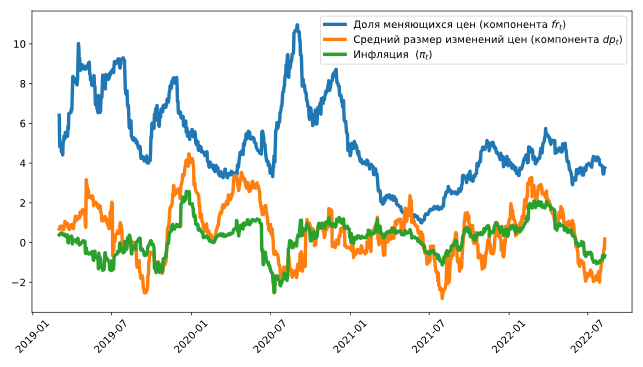
\includegraphics[width=\textwidth]{inflation_decompose}
	\caption{Динамика инфляции и ее компонент}
	\label{fig:inflation_decompose}
\end{figure}

Для оценки взаимосвязи динамики инфляции и её отдельных компонентов на исследуемой выборке были построены две регрессионные модели. В первой инфляция выступает в роли объясняющей переменной, а компонент $\textit{fr}_{t}$ – в роли объясняемой (уравнение (\ref{eq:regression__1})). Во второй модельной зависимости инфляция объясняет компонент $\textit{dp}_{t}$ (уравнение (\ref{eq:regression__2})):

\begin{equation}
	\textit{fr}_{t} = \alpha_{fr} + \beta_{fr} \cdot \pi_{t} + \epsilon_{t}
	\label{eq:regression__1}
\end{equation}

\begin{equation}
	\textit{dp}_{t} = \alpha_{dp} + \beta_{dp} \cdot \pi_{t} + \nu_{t}
	\label{eq:regression__2}
\end{equation}

Результаты оценивания регрессионных моделей (\ref{eq:regression__1}) и (\ref{eq:regression2}) представлены в таблице \ref{tab:regression_period_results}, где приводятся данные как для всего периода анализа, так и для отдельных подпериодов. Анализ показывает, что за весь период значимой является связь между инфляцией и компонентом $\textit{fr}_{t}$, что соответствует гипотезе о временно-зависимых моделях ценообразования. Аналогичная картина наблюдается и в подпериодах 1–3 (с февраля 2019 г. по 24 февраля 2022 г.). Однако, начиная с периода после 24 февраля 2022 г., статистически значимыми становятся оценки для связи инфляции с компонентом $\textit{dp}_{t}$.

Эти результаты объясняются тем, что после 24 февраля 2022 г. уровень годовой инфляции превысил пороговое значение в 10\%. Согласно эмпирическим выводам, представленным в работе \cite{gagnon2009}, преодоление этого порога усиливает корреляцию между инфляцией и средним размером изменений цен (компонент $\textit{fr}_{t}$), а также между инфляцией и долей товаров с меняющимися ценами (компонент $\textit{dp}_{t}$).

\begin{table}[h]
	\centering
	\small % Уменьшение размера шрифта
	\caption{Результаты оценок $\beta_{fr}$ и $\beta_{dp}$ из уравнений \ref{eq:regression__1} и \ref{eq:regression__2} соответственно}
	\label{tab:regression_period_results}
	\begin{tabularx}{\textwidth}{|X|X|X|X|X|X|}
		\hline
		\multirow{2}{*}{\textbf{Период}} & \textbf{Весь период} & \multicolumn{4}{c|}{\textbf{Отдельные подпериоды}} \\
		\cline{3-6}
		& (2019–2022 гг.) & 1. Год до COVID-19 (февраль 2019 – февраль 2020) & 2. Год начала COVID-19 (март 2020 – февраль 2021) & 3. Год после COVID-19 (март 2021 – февраль 2022) & 4. После 24 февраля 2022 (март 2022 – сентябрь 2022) \\
		\hline
		$\beta_{fr}$ & 0,4 & -2,1 & -2,2 & 1,6 & 9,3*** \\
		\hline
		$\beta_{dp}$ & 7,8*** & 18,1*** & 13,3*** & 13,5*** & 9,2*** \\
		\hline
	\end{tabularx}
	\begin{tablenotes}
		\item \textbf{Примечание:} *** – статистическая значимость на 1\% уровне.
	\end{tablenotes}
\end{table}




